\chapter{Implementation of domain modeling assistant}

TODO: Brief chapter description.


\section{Generators configuration}

TODO: Provide reference for our GitHub prompts directory reference\footnote{\url{https://github.com/Dominik7131/Conceptual-Modeling-LLM-Assistant/tree/master/prompts}}

TODO: V nějaké sekci pak říct, že jsme iterativní techniky nedělali


\subsection{Output order}
\label{output_order}

When the task of modeling domain elements solely based on a given domain description is done by the modeling experts, they typically proceed in the following two steps: (1) they find the context for the given element and (2) from the found context they extract the specific information such as name of the element.

To mimic this approach, we instruct the LLM in the output specification part to first generate the context for the given element and then to generate the specific information of this element.


\subsection{Output specification}
We insert each structured data in the JSON format as each LLM should be greatly familiar with this format. To improve the response time of our application we instruct the LLM to output one isolated JSON object for each outputted domain element. This way as soon as the LLM generates some proper domain element it can be displayed to the user.


\subsection{Modeling procedure}

TODO: Provide examples for each prompting technique


\subsubsection{Chain of thoughts}

Implementing CoT strategy for generating domain elements is a challenging task as this process does not contain any straightforward steps. As described in the section \ref{output_order} about output order we already instruct the LLM to find the context first and then the specific information.

When an instruction such as ``Think step by step'' is inserted into the prompt, the LLM outputs only the corresponding domain elements in the specified output format without any reasoning. \\

TODO: Example ChatGPT-4o with a simple domain description from for example domain modeling steps \\

To put more emphasis on generating the context first of the corresponding domain element, we came up with a simple CoT strategy that instructs the LLM to generate output for each domain element step by step. \\

Other more sophisticated CoT strategies can be used. For example, when the LLM generates attributes to instruct the LLM to add for each generated domain element a reason why it thinks it is an attribute. \\

TODO: Example ChatGPT-4o + as before but with our simple CoT \\


TODO: Odůvodnit proč jsme nedělali iterativní generování, kde by ještě LLM třeba zhodnotil každý vygenerovaný výstup (důvod: chceme responzivní aplikaci)


\subsubsection{N-shot prompting}

We use examples based on the domain description and its domain model that is shown in the figure \ref{fig:prompting-domain}.

\begin{figure}[!h]
    \centering
    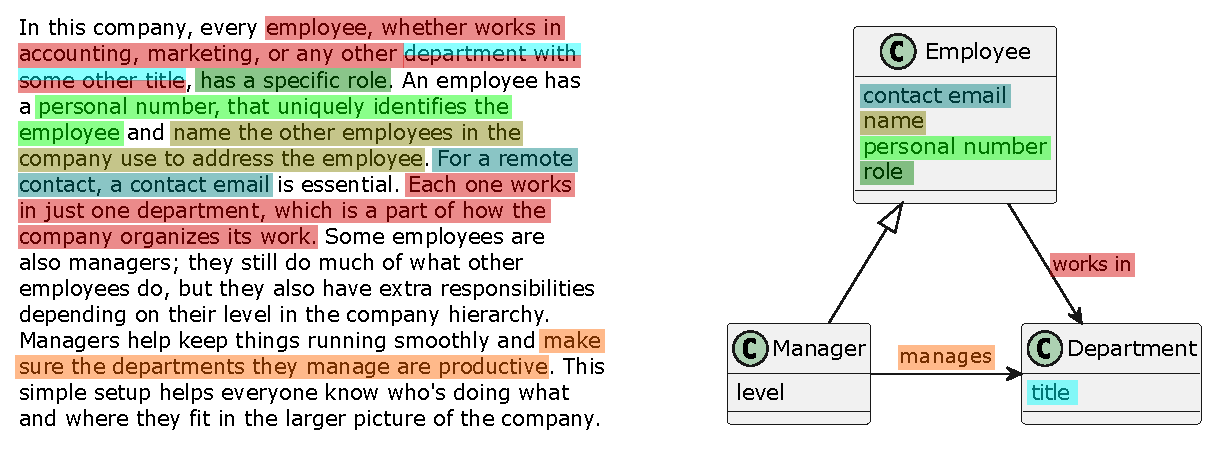
\includegraphics[scale=0.6]{img/prompting-domain.pdf}
    \caption{\centering The simple company employees domain description and its corresponding domain model used for N-shot prompting in our generator templates}
    \label{fig:prompting-domain}
\end{figure}


For $gen_c$, we use the three classes as examples. For $gen_a$, we use the colored attributes, each with the colored part of the text as examples of the corresponding original texts. For $gen_{r1}$ and ${gen_{r2}}$, we proceed similarly, but for ${gen_{r1}}$ we provide each sample association twice – for the source class and for the target class.

The concrete examples can be used to further specify the output format. For example,  when the LLM is not provided with a specific name format of the corresponding domain elements, the outputted names can sometimes be in a snake case convention and some other time in a camel case convention. When the provided examples contain a consistent naming format the LLM outputs the provided format consistently. Similarly, this helps to specify the naming style. For example without providing any naming style some generated attributes can contain some unwanted words such as the word ``has'' at the start of the attribute.


\subsubsection{Tree of thoughts}

TODO: Myšlenka taková, že pro zadanou úlohu necháme LLM vygenerovat několik seznamů odpovídajících domain elementů. A potom s těmi elementy provedeme nějakou operaci, jako například sjednocení a všechny dáme na výstup, nebo uděláme jejich průnik, nebo necháme LLM hlasovat pro každý element atd.

TODO: asi to motivovat to tím, že naše preliminary experimenty ukázaly, že CoT zlepšuje kvalitu výstupu LLM (ale pak ve výsledku jsme to stejně nezměřili pro atributy a asociace, takže to asi není dobrý argument)


\subsection{Retrieval-augmented generation}

We consider the domain description $T$ as the knowledge base and our goal is to insert only the relevant parts of the $T$ in the context specification part of the prompt. We use this technique for the generators of: attributes, associations, descriptions, data types and cardinalities as in these cases only the information about the source class $C$ is needed for generating correct output.

For example, if in domain description the first sentence informs us about employees and the second sentence informs us about projects, when suggestion attributes for the class ``employee'' we insert only the first sentence in the prompt. This is mainly done to reduce the hallucination of the LLM such as reducing irrelevant domain elements suggestion by focusing on the important parts of the domain description. Furthermore, this approach also usually reduces the prompt length when working with a domain description that does not fit into the context window size of the LLM. \\

TODO: Specific example instead of only example description

Now we describe the most significant challenges we encountered and the corresponding solutions we implemented to address them.


\subsubsection{Domain description pre-processing}

We considered using a LLM to pre-process the domain description by simplifying it's sentences in the first step. However, the LLM usually changes some of the names of the domain element or completely removes some domain elements which would lead to LLM generated suggestions containing a different domain element names than in the original domain description. Furthermore, pre-processing the domain description complicates highlighting of the suggested domain elements in the original provided domain description. Therefore, we do not pre-process the domain description. \\

TODO: Example - v promptu LLM říct, ať nemění jména žádných domain elementů a ať je výsledek v jednoduchých větách a možná pak ještě, že informace ať se neopakují (ale nejdřív to zkusit klidně s opakováním informací).


\subsubsection{Domain description segmentation}

First, the domain description needs to be split into chunks so each chunk can be evaluated if it is relevant for the given source class.

Determining the chunk size is a challenging task since with too big chunks we are risking having irrelevant parts of domain description in the prompt and thus decreasing the LLM performance. On the other hand, with too small chunks we are risking that the chunks will be miss-classified as they will not contain enough information about their context for deciding if they are relevant.

In result, we consider each sentence of the domain description as one chunk since one sentence usually contains information about one concept or a few related concepts. Additionally, later on it is easy to concatenate the relevant chunks together simply by putting them next to each other in the original order from the domain description.


\subsubsection{Texts comparison}
\label{texts_comparison}
  
We considered using LLM to directly output the relevant texts from the domain description based on the given source class. However, this process can take many seconds as in the worst case scenario the LLM has to copy the whole domain description to the output.

Instead, we implemented a semantic and a syntactic approach that for a given source class and some part of a domain description compares their similarity.
 
The semantic approach uses an embedding model that converts input texts into a vector space and then compares their similarity.

The syntactic approach compares lemmas of the mentioned texts. As one word in a different contexts can have a different lemmas, we lemmatize each word by word in isolation. \\

TODO: Více rozepsat, jakým způsobem to syntaktické filtrování funguje + na jaké problémy jsem narazil + příklady


\subsubsection{Top k search}

In traditional RAG systems, a fixed number $k$ of the most relevant results are retrieved after applying the embedding model. However, in our specific application, $k$ is not a fixed number because the domain description may contain a variable number of relevant sentences. To address this variability, we need to set the computed score threshold. The challenge lies in the fact that the computed score is always relative to the given input. Consequently, in one scenario, sentences with a score higher than a certain threshold $x$ may be considered relevant, while in another scenario, sentences with a score higher than $x$ may be considered irrelevant.

We found out that our semantic RAG approach works a little bit better when setting the threshold based on the score of the most relevant sentence. For more information see the RAG evaluation section (TODO: section reference).


\subsubsection{Lack of context}

Our segmentation into sentences can fail when for example some sentence contains pronoun referencing anything from a previous sentence. For example consider this domain description: ``The book contains a lot of pages. It is very heavy.'' and input class named ``book''. Now when considering only the second sentence it does not contain any syntactic information about the book therefore it most probably would be discarded by any syntactic or semantic comparison algorithm even thought for example the attribute \textit{weight} of the class \textit{book} could be derived from it.

One possible solution is to use some language model that can accurately solve the co-reference resolution task where each pronoun is replace with the corresponding words that are referenced. This way the previous example would look like this: ``The book contains a lot of pages. The book is very heavy.''

However, we did not find any working model with a high accuracy for a various domain descriptions so instead, we implemented a simple naive solution where each sentence has it's own metadata. If a sentence starts with a pronoun we insert in this metadata a reference into the previous sentence. This means that when some algorithm is testing relevancy of the sentence ``It is very heavy''. In reality it is testing relevancy of this sentence and also the previous sentence ``The book contains a lot of pages.''

Similar issue can arise when a text contains some bullet point, such as: \\

``The book contains:
\begin{itemize}
\item info about it's author
\item date of publication''
\end{itemize}

In this case each of the bullet points will have in it's metadata reference to the sentence before the first bullet points which in this case is ``The book contains:'' and the problem is solved.

However, other issues can appear such as unexpressed subject. If the main goal of the assistant is to always suggest all possible domain elements then either the RAG can be temporarily disabled or each domain description have to be manually pre-processed first to remove the mentioned issue. Otherwise, the problematic domain element can be manually modeled by the user.